\documentclass[a4paper,11pt]{article}
\usepackage[utf8]{inputenc}
\usepackage{graphicx}
\usepackage[english]{babel}
\usepackage[vmargin=3.5cm, top=2cm]{geometry}
\usepackage[linktocpage=true]{hyperref}
\usepackage{enumitem}
\usepackage{longtable}
\usepackage{pdfpages}
\usepackage{float}
\usepackage{hyperref}
\usepackage[section]{placeins}
\hypersetup{
   colorlinks,
   citecolor=black,
   filecolor=black,
   linkcolor=black,
   urlcolor=black
}

\begin{document}

\begin{titlepage}

\centering \parindent=0pt
\newcommand{\HRule}{\rule{\textwidth}{1mm}}
\vspace*{\stretch{1}} \HRule\\[1cm]\Huge\bfseries
Data Mining Report\\[0.7cm]
\HRule\\[4cm]  
\large by 
\\ Mikkel Stolborg
\\ Hlynur Örn Haraldsson
\vspace*{\stretch{2}} \normalsize %
\begin{flushleft}
IT University of Copenhagen \\
MDMI, S2015\\
Anders Hartvig Hartzen\\
Hajira Jabeen\\
Héctor Pérez Martínez\\
Sebastian Risi\\
Noor Shaker\\
\today \end{flushleft}
\end{titlepage}

\tableofcontents
\pagebreak
\section{Introduction}
\subsection{Data selection}
We have worked on a data set regarding the passengers on the titanic. The data structure is presented in table \ref{titanData} with a short name and the value type associated with the variable. 
The type binary and binary string, means there is only two options, the first of the types is based on numeric binary data, whilst the second is based on string data. The value type attribute table covers three options. The 
\begin{table}[h]
\begin{tabular}{|l|l|l|}
\hline
Variable name & Short name & Value Type\\
\hline
survival & Survived & binary\\
pclass & Passenger Class & numeric\\
name & Name & string\\
sex & Sex & binary string\\
age & Age & numeric\\
sibsp & Number of Siblings/Spouses Aboard & numeric\\
parch & Number of Parents/Children Aboard & numeric\\
ticket & Ticket Number & string\\
fare & Passenger Fare & numeric\\
cabin & Cabin & string\\
embarked & Port of Embarkation & attribute table\\
\hline
\end{tabular}
\caption{Titanic data set variables with short description and classification.}
\label{titanData}
\end{table}

VARIABLE DESCRIPTIONS:
survival        Survival
                (0 = No; 1 = Yes)
pclass          Passenger Class
                (1 = 1st; 2 = 2nd; 3 = 3rd)
name            Name
sex             Sex
age             Age
sibsp           Number of Siblings/Spouses Aboard
parch           Number of Parents/Children Aboard
ticket          Ticket Number
fare            Passenger Fare
cabin           Cabin
embarked        Port of Embarkation
                (C = Cherbourg; Q = Queenstown; S = Southampton)

SPECIAL NOTES:
Pclass is a proxy for socio-economic status (SES)
 1st ~ Upper; 2nd ~ Middle; 3rd ~ Lower

Age is in Years; Fractional if Age less than One (1)
 If the Age is Estimated, it is in the form xx.5

With respect to the family relation variables (i.e. sibsp and parch)
some relations were ignored.  The following are the definitions used
for sibsp and parch.

Sibling:  Brother, Sister, Stepbrother, or Stepsister of Passenger Aboard Titanic
Spouse:   Husband or Wife of Passenger Aboard Titanic (Mistresses and Fiances Ignored)
Parent:   Mother or Father of Passenger Aboard Titanic
Child:    Son, Daughter, Stepson, or Stepdaughter of Passenger Aboard Titanic

Other family relatives excluded from this study include cousins,
nephews/nieces, aunts/uncles, and in-laws.  Some children travelled
only with a nanny, therefore parch=0 for them.  As well, some
travelled with very close friends or neighbors in a village, however,
the definitions do not support such relations.
\subsection{Research question}
Our primary question which we want answered was:\\
\textit{"Which attributes contributes mostly to the survival rate of a passenger on the Titanic}\\
Here we wished to figure out what set of parameters would ensure the highest rate of survival on the Titanic. We would use classification through a classification tree to figure out which set gives the highest percentage of survival.

The secondary question arose when looking at clusters of the data.\\
\textit{"Which societal data can be found in clusters of the titanic data"}\\
Looking at the data, we decide to try clustering to see if there was an emergent pattern. It would be interesting to see if the were a relation between wealth and number of children and the like. 
\subsection{Tools for data mining}
We choose to use the free tool called Orange\cite{orange}. This tool allowed to quickly manipulate the data, such that we could extract the interesting elements. 
In the tool you manipulate the data by clicking and drawing connections between data elements and processing methods. Before explaining further, we have included the map of the process used for our data set in the orange framework, see figure \ref{OrangeMap}.

\begin{figure}[h]
	\centering
	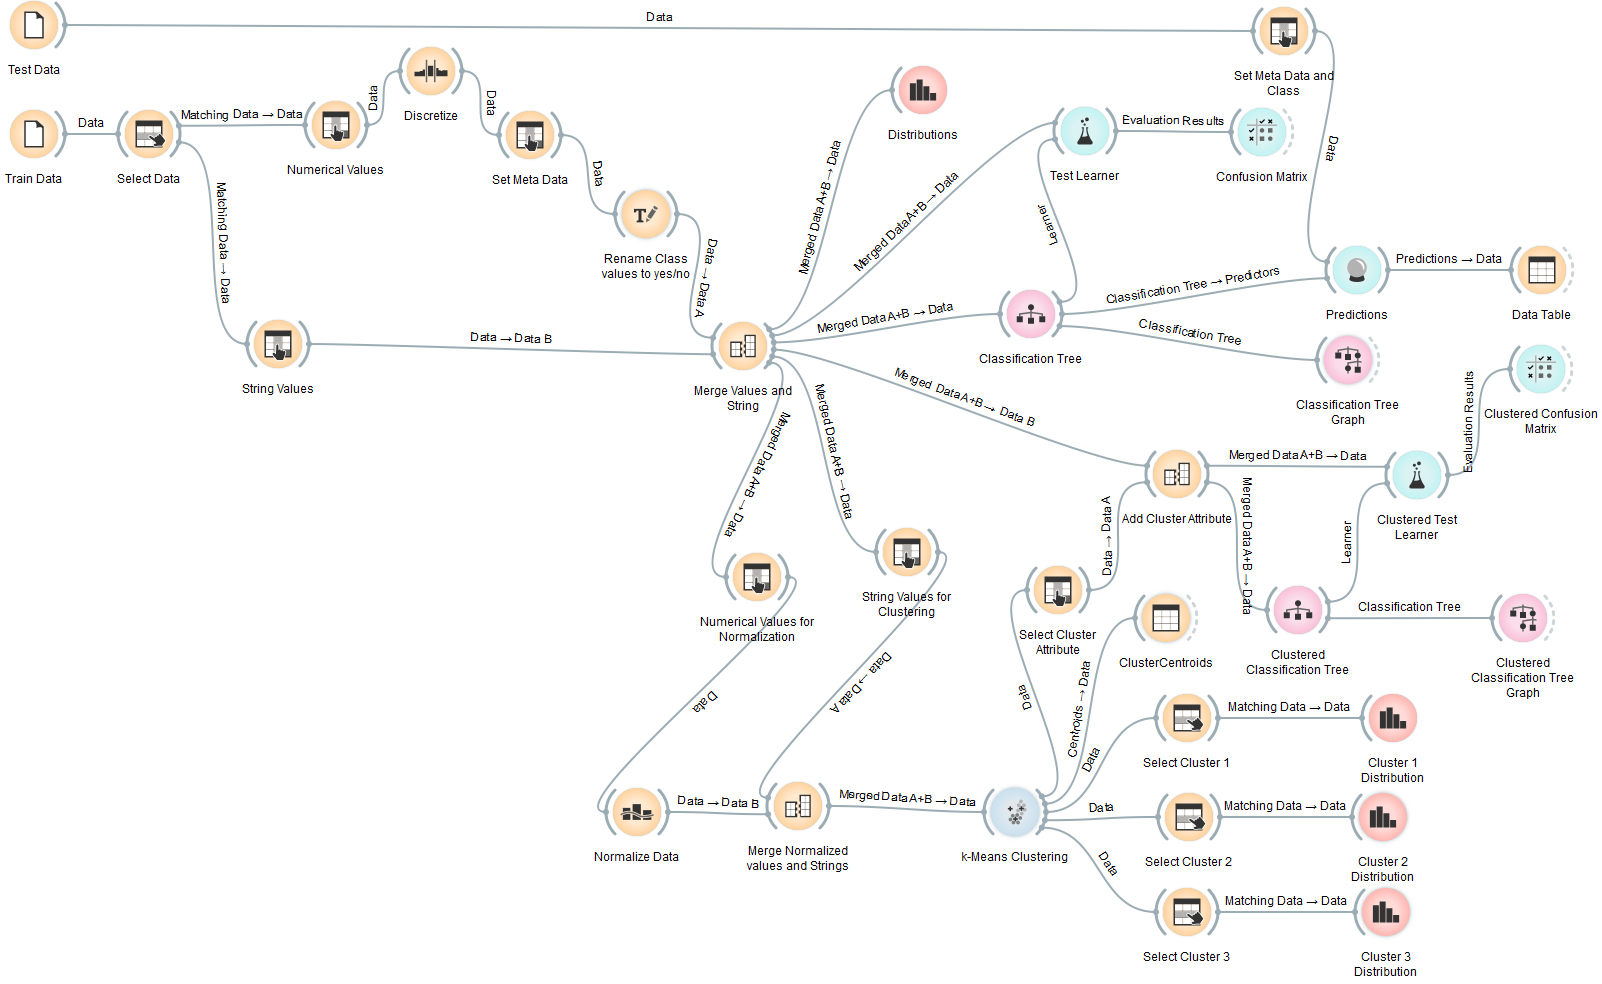
\includegraphics[scale=0.35]{orangeMap}
	\caption{The map of the methods and processes used on the data.}
	\label{OrangeMap}
\end{figure}


\section{Data mining}
\subsection{Preprocessing}
\subsection{Classification tree}
\subsubsection{Cross Validation}
\subsection{K-means Clustering}
\subsubsection{Data validation}

\section{Conclusion}
\subsection{Societal impact}




\appendix
\begin{thebibliography}{9}

\bibitem{orange}
  \emph{Orange Data Mining},
  http://orange.biolab.si/,
  13-05-15
\end{thebibliography}

\end{document}


